\subsection{Referring expression generation}
\label{sec:referring-expression-generation-game}
\subsubsection*{Setup}

In a next step, it is tested if the agents can learn to extract features of the objects together.
For this the same sender as in the previous section is used.
Based on the results, $h_s$ is fixed to $500$ and $e_s$ to $100$.
However, the task and by that the receiver's architecture is adapted in two different ways.
In the first setup, the \textbf{referring expression generator}, the receiver is tasked to describe the target object with natural language following the \emph{incremental GRE-algorithm} based on the sender's message (see Figure \ref{fig:caption_generator_game_architecture}).
This follows the approach of the approach of the \emph{RE generators} described in Section \ref{sec:referring_expression_generation}.
The whole scene is encoded using the \emph{image encoder} submodule, projecting it to the image encoding dimension $e_{ri}=100$.
The sender's message is decoded with the hidden size $h_r=500$ and $e_r=100$, and concatenated with the encoded image.
This is then reduced to $LSTM_o=1500$ dimensions based on the results of the previous experiments, and used as the initial state of the captioning LSTM.
Tokens are embedded with $LSTM_e=15$ dimensions.
Since the position of the padding as well as the order of the words in the target didn't have an effect on the results, the usual approach in natural generation task is used: padding tokens are appended and the referring expression is not reversed.
During training, the ground truth caption is used as the input to the LSTM using teacher forcing.
% SD: I'm not sure how teacher forcing is implemented, see my earlier comment
% DK: typo, teacher forcing is actually applied (done)
When presented with test data, the LSTM always produces three tokens, by using its own predicted words as the input for the next step.
The loss is calculated using cross entropy.

\begin{figure}[ht]
    \centering
    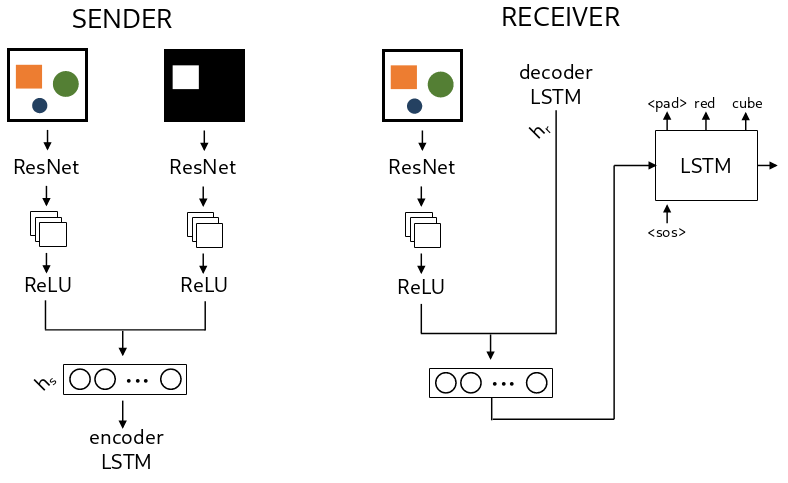
\includegraphics[width=.7\linewidth]{figures/arch_caption_generator_game.png}
    \caption{Simplified architecture of the referring expression generator game}
    \label{fig:caption_generator_game_architecture}
    % SD: But here we don't need an LSTM, we just want to identify one of the objects. The LSTM should only encode the inout message.
    % DK: TODO
\end{figure}

However, this setup could lead to two problems:
First, the task is quite complex for both agents to learn, since two language generation steps are involved.
This might stop the agents from converging towards a useful language.
Secondly, in case a language emerges, it could be aligned with the natural language of the target referring expressions.
In other words, the sender might just learn to effectively repeat the target referring expressions without extracting the necessary features themselves.
For that reason, in the second setup, the \textbf{attribute generator} the receiver is tasked to predict only the attributes of the target object in the shape of a multi-hot vector (shown in Figure \ref{fig:attribute_generator_game_architecture}).
By this, no natural language including its salience order is involved and the complexity of the complete game is reduced.
The receiver uses the same way to encode and combine the complete scene and the sender's message with $e_{ri}=100$, $h_r=500$ and $e_r=100$.
This is then passed to a linear layer that produces a vector with 13 dimension, corresponding to the 2 sizes, 3 shapes, and 8 colors.
The loss is then calculated using binary cross entropy.

\begin{figure}[ht]
    \centering
    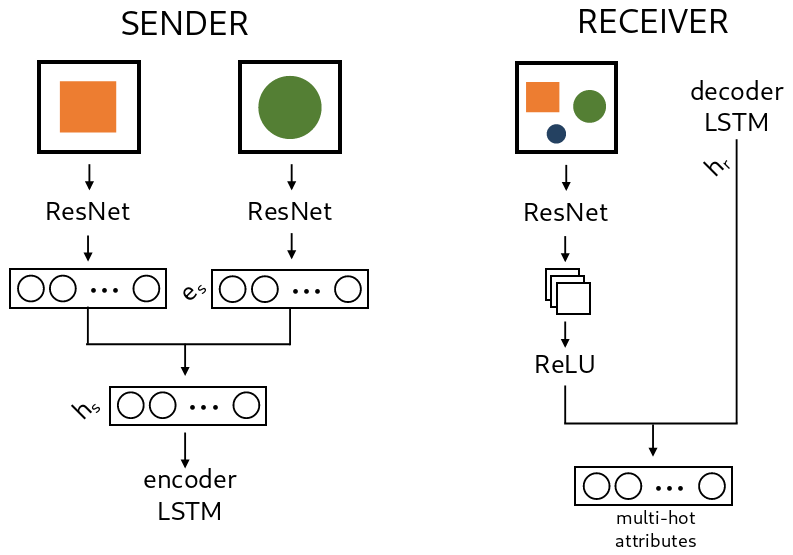
\includegraphics[width=.55\linewidth]{figures/arch_attribute_generator_game.png}
    \caption{Simplified architecture of the attribute generator game}
    \label{fig:attribute_generator_game_architecture}
\end{figure}

The experiments for both setups are conducted with a learning rate of $2\times10^{-4}$.
As in the previous section, the following values for the variables are compared:
\begin{itemize}
    \item $|V|$: 2, 10, 16, 50, 100
    \item $n$: 1, 2, 3, 4, 6
\end{itemize}

Since the agents are trained to describe the target object discriminatively based on the described GRE-algorithm, they are trained on the 'Dale-2', 'Dale-5' and 'CLEVR color' dataset.
The 'Dale-5' and the 'CLEVR color' should be again much harder to learn, since there are more objects that the agents need to discriminate the target object from.
% SD: So the sender is generating descriptions following the GRE policy?
% DK: TODO
The same metrics as in the Section \ref{sec:referring_expression_generation} are used to evaluate the results for the first setup.
When predicting multi-hot vectors, an overall \textbf{accuracy} is reported that reflects if all attributes were predicted correctly.
Additionally, the accuracy for each attribute is calculated separately to show which attributes give bigger challenges for the models.

\subsubsection*{Results}
\begin{figure}[ht!]
    \centering
    \subfigure['Dale-2' dataset with different $|V|$ highlighted]{
        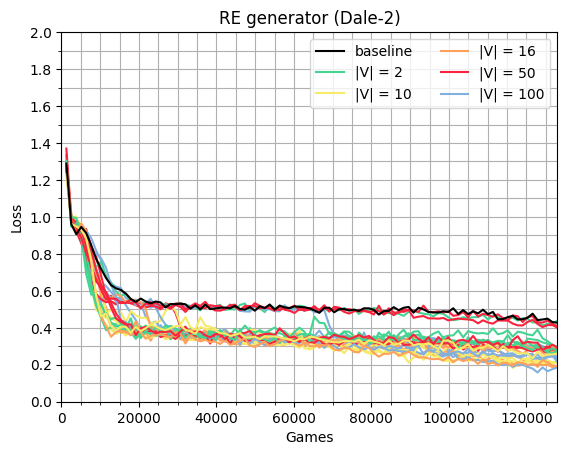
\includegraphics[width=0.485\linewidth]{figures/learning-curve_re-generator_dale-2_vocab-size.png}
        \label{fig:learning-curve_re-generator_dale-2_vocab-size}
    }
    \subfigure['Dale-2' dataset with different $n$ highlighted]{
        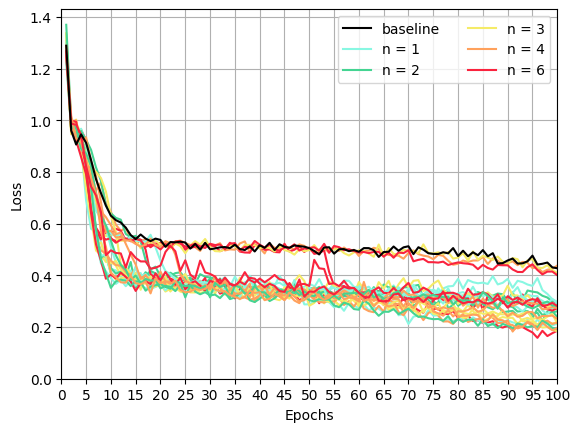
\includegraphics[width=0.485\linewidth]{figures/learning-curve_re-generator_dale-2_max-len.png}
        \label{fig:learning-curve_re-generator_dale-2_max-len}
    }
    \subfigure['Dale-5' dataset with different $|V|$ highlighted]{
        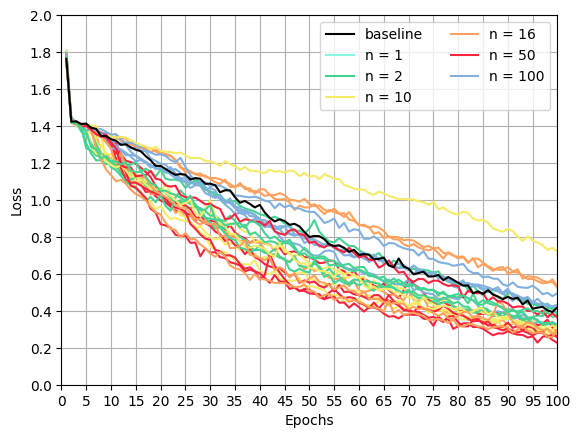
\includegraphics[width=0.485\linewidth]{figures/learning-curve_re-generator_dale-5_vocab-size.png}
        \label{fig:learning-curve_re-generator_dale-5_vocab-size}
    }
    \subfigure['Dale-5' dataset with different $n$ highlighted]{
        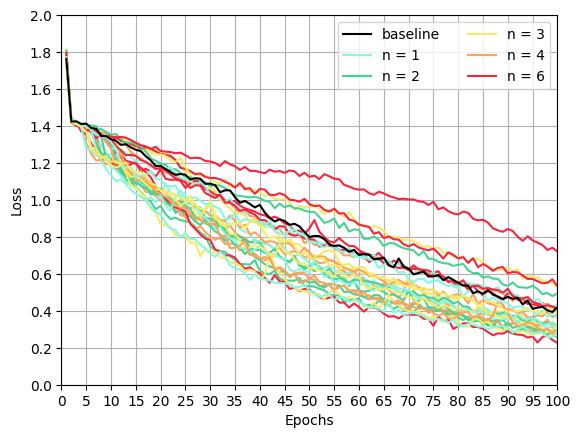
\includegraphics[width=0.485\linewidth]{figures/learning-curve_re-generator_dale-5_max-len.png}
        \label{fig:learning-curve_re-generator_dale-5_max-len}
    }
    \caption{Learning curves of all referring expression generation games on the \emph{Dale} datasets. On the 'CLEVR color' dataset, the learning curves don't diverge from the baseline and are therefore left out. In the left column, the colors correspond to different vocabulary sizes $|V|$ while in the right column, the colors correspond to different message lengths $n$. The baseline is marked in black.}
    \label{fig:learning-curves_re-generator}
\end{figure}

As in the previous section, Figure \ref{fig:learning-curves_re-generator} shows the learning curves of all configurations of the \textbf{referring expression generator}.
The baselines are shown in black.
Hereby, the sender is sending random messages, so that the receiver needs to solve the task on their own.
In all configurations that don't pass this baseline, no meaningful messages are exchanged, and no language emerged.
If configurations perform better on the other hand means that the agents learned to encode some meaning in their messages.
While for both \emph{Dale} dataset, several configuration diverge from the baseline, in other words, learning takes place, all learning curves align with the baseline for the 'CLEVR color' dataset and are therefore left out.
Looking at the learning curves for the 'Dale-2' dataset, most of the configurations can decrease the loss compared to the baseline faster on to a bigger extend.
Fast learning takes place in the first 10.000 to 15.000 games and decelerates afterwards.
Also on this task, there are several configurations that converge much later than the initial fast decrease of the loss.
Most of these configurations diverge from the baseline between 15.000 to 35.000 games, but some even need up to 70.000 games.
While the vocabulary size now seems to have a lower impact on the learning speed, configurations that converge later tend to have a message length of $n=6$.
For the 'Dale-2' dataset a clear distinction between configurations that align with the baseline and configurations that diverge from the baseline is visible.
For the 'Dale-5' dataset, however, all learning curves are closer together and success of learning is not instantly apparent.
Nonetheless, several configurations (with low- to medium-sized vocabularies) start to converge earlier than the baseline.
Configurations with $|V|=2$ start to do so already after 5.000 games, with $|V|\in\{10,16\}$ after around 7.000 games and with $|V|=50$ after around 12.000 games.
With $|V|=100$, almost no configuration diverges from the baseline.
The message length doesn't seem to have an impact.
Interestingly, there are several configurations that perform worse than the baseline, and communication between the agents seems to hinder the learning.
This happens across all vocabulary sizes and message lengths.

\begin{table}[ht]
    \centering
    \begin{tabular}{cc|ccc|ccc|ccc}
        \toprule
                                      &        & \multicolumn{3}{c}{\textbf{Dale-2}} & \multicolumn{3}{c}{\textbf{Dale-5}} & \multicolumn{3}{c}{\textbf{CLEVR color}}                                                                                                                                                       \\  \cmidrule(lr){3-5}\cmidrule(lr){6-8}\cmidrule(lr){9-11}
        $n$                           & $|V|$  & \textbf{Acc.}                       & \textbf{F1}                         & \textbf{NT}                              & \textbf{Acc.}          & \textbf{F1}            & \textbf{NT}            & \textbf{Acc.}          & \textbf{F1}            & \textbf{NT}            \\\midrule
        \multicolumn{2}{c|}{baseline} & {41,8} & {42,36}                             & {37,11}                             & {62,66}                                  & {81,16}                & {18,36}                & {13,52}                & {33,08}                & {34,53}                                         \\\midrule
        {1}                           & {2}    & {70,49}                             & {54,73}                             & {7,29}                                   & {70,16}                & {85,06}                & {13,06}                & \textcolor{red}{11,68} & \textcolor{red}{32,25} & \textcolor{red}{34,03} \\
        {1}                           & {10}   & {78,26}                             & {63,33}                             & {3,56}                                   & {68,97}                & {85,01}                & {10,85}                & \textcolor{red}{12,72} & \textcolor{red}{32,77} & \textcolor{red}{33,85} \\
        {1}                           & {16}   & {74,18}                             & {52,21}                             & {5,38}                                   & {71,57}                & {86,87}                & {10,72}                & \textcolor{red}{13,19} & \textcolor{red}{33,64} & \textcolor{red}{33,33} \\
        {1}                           & {50}   & {70,83}                             & \textcolor{red}{43,56}              & {4,21}                                   & {65,23}                & {83,11}                & {12,54}                & \textcolor{red}{11,81} & \textcolor{red}{33,14} & \textcolor{red}{34,72} \\
        {1}                           & {100}  & {73,18}                             & {52,14}                             & {3,86}                                   & \textcolor{red}{60,94} & \textcolor{red}{80,85} & \textcolor{red}{20,36} & \textcolor{red}{13,67} & \textcolor{red}{33,71} & \textcolor{red}{33,64} \\
        {2}                           & {2}    & {72,31}                             & {50,42}                             & {5,52}                                   & {66,2}                 & {83,39}                & {14,42}                & \textcolor{red}{13,32} & \textcolor{red}{33,62} & \textcolor{red}{32,73} \\
        {2}                           & {10}   & {75,22}                             & {58,4}                              & {3,99}                                   & {73,22}                & {87,68}                & {9,03}                 & \textcolor{red}{12,37} & \textcolor{red}{33,3}  & \textcolor{red}{34,11} \\
        {2}                           & {16}   & {\textbf{81,64}}                    & {\textbf{73,66}}                    & {\textbf{2,86}}                          & {73,44}                & {88,21}                & {8,85}                 & \textcolor{red}{12,98} & \textcolor{red}{33,94} & \textcolor{red}{34,24} \\
        {2}                           & {50}   & {74,39}                             & {48,53}                             & {3,17}                                   & {\textbf{75,35}}       & \textbf{88,77}         & \textbf{8,07}          & \textcolor{red}{14,19} & \textcolor{red}{33,04} & \textcolor{red}{33,46} \\
        {2}                           & {100}  & {74,09}                             & {54,88}                             & {3,65}                                   & \textcolor{red}{54,56} & \textcolor{red}{76,95} & \textcolor{red}{22,57} & \textcolor{red}{13,28} & \textcolor{red}{32,8}  & \textcolor{red}{33,38} \\
        {3}                           & {2}    & {71,03}                             & {50,76}                             & {4,62}                                   & {65,18}                & \textcolor{red}{82,68} & {14,23}                & \textcolor{red}{12,76} & \textcolor{red}{33,58} & \textcolor{red}{33,64} \\
        {3}                           & {10}   & {76,91}                             & {59,42}                             & {2,6}                                    & {71,66}                & {87,14}                & {9,9}                  & \textcolor{red}{12,54} & \textcolor{red}{32,75} & \textcolor{red}{33,85} \\
        {3}                           & {16}   & {79,95}                             & {67,55}                             & {3,17}                                   & \textcolor{red}{50,13} & \textcolor{red}{73,24} & {24,22}                & \textcolor{red}{12,93} & \textcolor{red}{33,79} & \textcolor{red}{34,46} \\
        {3}                           & {50}   & {62,93}                             & {48,03}                             & {16,58}                                  & {\textbf{76,09}}       & {\textbf{88,5}}        & \textbf{9,2}           & \textcolor{red}{13,67} & \textcolor{red}{33,73} & \textcolor{red}{34,29} \\
        {3}                           & {100}  & {75,74}                             & {57,51}                             & {2,43}                                   & {69,7}                 & {86,14}                & {9,38}                 & \textcolor{red}{13,02} & \textcolor{red}{33,64} & \textcolor{red}{34,2}  \\
        {4}                           & {2}    & \textcolor{red}{41,23}              & \textcolor{red}{42,53}              & \textcolor{red}{35,33}                   & {63,93}                & \textcolor{red}{82,34} & {15,3}                 & \textcolor{red}{12,2}  & \textcolor{red}{33,25} & \textcolor{red}{33,64} \\
        {4}                           & {10}   & {78,99}                             & {66,4}                              & {2,08}                                   & {73,22}                & {88,01}                & {10,85}                & \textcolor{red}{12,5}  & \textcolor{red}{33,55} & \textcolor{red}{33,16} \\
        {4}                           & {16}   & {\textbf{80,08}}                    & {\textbf{70,48}}                    & {\textbf{3,47}}                          & {69,4}                 & {86,09}                & {10,63}                & \textcolor{red}{11,72} & \textcolor{red}{33,1}  & \textcolor{red}{34,03} \\
        {4}                           & {50}   & {75,48}                             & {54,44}                             & {3,34}                                   & {71,35}                & {86,61}                & {10,68}                & \textcolor{red}{11,81} & \textcolor{red}{33,18} & \textcolor{red}{34,33} \\
        {4}                           & {100}  & {74,78}                             & {57,09}                             & {3,86}                                   & \textcolor{red}{59,2}  & \textcolor{red}{80,14} & \textcolor{red}{20,57} & \textcolor{red}{12,67} & \textcolor{red}{32,3}  & \textcolor{red}{34,55} \\
        {6}                           & {2}    & {72,87}                             & {51,44}                             & {2,78}                                   & {60,82}                & \textcolor{red}{80,42} & {17,07}                & \textcolor{red}{13,45} & \textcolor{red}{33,73} & \textcolor{red}{33,64} \\
        {6}                           & {10}   & {73,61}                             & {48,73}                             & {2,82}                                   & \textcolor{red}{32,64} & \textcolor{red}{58,42} & \textcolor{red}{33,12} & \textcolor{red}{11,89} & \textcolor{red}{33,15} & \textcolor{red}{35,03} \\
        {6}                           & {16}   & {73,52}                             & {49,67}                             & {2,43}                                   & \textcolor{red}{49,39} & \textcolor{red}{73,19} & \textcolor{red}{23,78} & \textcolor{red}{13,06} & \textcolor{red}{32,31} & \textcolor{red}{34,64} \\
        {6}                           & {50}   & \textcolor{red}{44,31}              & {45,07}                             & \textcolor{red}{33,29}                   & {\textbf{78,82}}       & {\textbf{90,22}}       & {\textbf{7,29}}        & \textcolor{red}{12,72} & \textcolor{red}{33,29} & \textcolor{red}{32,99} \\
        {6}                           & {100}  & {\textbf{80,95}}                    & {\textbf{69,88}}                    & {\textbf{3,34}}                          & {62,2}                 & \textcolor{red}{80,62} & \textcolor{red}{19,88} & \textcolor{red}{14,24} & \textcolor{red}{32,36} & \textcolor{red}{32,94} \\
        \bottomrule
    \end{tabular}
    \caption{Overall accuracies (Acc.), F1-score (F1) and non-target accuracies (NT) in \% of the RE generator after 128.000 games: $n$ are different maximum message lengths and $|V|$ are different vocabulary sizes.}
    \label{tab:results:re-generator-game}
\end{table}

Table \ref{tab:results:re-generator-game} shows the \emph{overall accuracies}, \emph{F1-scores} and \emph{non-target accuracies} across all datasets for different message lengths $n$ and vocabulary sizes $|V|$.
When first having a look at the results of the 'Dale-2' dataset, it can be seen that the baseline already identifies correct referring expressions in 41,8\% of the samples.
However, almost all other configurations perform much better.
This shows that the agents consistently learn languages to solve the tasks.
Still, differences in how well the agents perform can be identified.
While a small vocabulary with $|V| = 2$ mostly beats the baseline, the emerged language only lets the agents generate the correct referring expression in a maximum of around 72\% of the samples.
The similar result is visible for a bigger vocabulary size of $|V|=50$ which has the highest accuracy at around 74\%.
A vocabulary size of $|V|=100$ performs consistently slightly better, with accuracies of around 73\% to 75\%.
Interestingly, when the agents are allowed to exchange messages with a message length of $n=6$, the accuracy peaks at almost 81\%.
Additionally, also the \emph{F1-score} almost reaches 70\% whereas it usually stayed around 50\% to 60\% in the previously discussed configuration.
The \emph{F1-score} evaluates each word in the referring expression separately instead of the binary \emph{overall accuracy} for the complete referring expression.
A small increase of the accuracy accompanied by a large increase of the F1-score indicates that the agents learned to encode an additional attribute, with the larger vocabulary and longer messages.
Finally, vocabulary sizes of $|V|=10$ and $|V|=16$ consistently perform the best with accuracies of 74\% to 81\%.
However, a difference in the \emph{F1-score} is visible: configurations with $|V|=16$ reach 67,55\% to 73,66\% with message lengths $n \in [2,4]$, where $|V|=10$ only reaches an F1-score of 66,4\% with $n=4$ and otherwise performs worse.
This indicates as before that the agents were able to encode more attributes with the larger vocabulary.

The results look different when the agents are trained to generate referring expressions for the 'Dale-5' dataset.
First, the baseline, in other words the receiver on their own, performs much better.
It already produces the whole correct referring expressions in 62,66\% of the samples, and achieves and \emph{F1-score} of 81,36\%.
However, the \emph{non-target accuracy} is quite high with producing correct referring expressions for a distractor in 18,36\% of the cases.
This allows two conclusions: On the one side, the baseline can pretty successfully extract a bias from the images.
Since there are multiple distractors in the image, the probability that they share attributes that are relevant for discriminating the target is higher.
The model therefore can learn to generate \emph{shapes} and \emph{colors} that appear more often correctly, which leads to a higher \emph{F1-score}.
On the other side, the larger number of distractors makes it possible for the model to single out the target from the image alone, as it needs to be uniquely identifiable.
If there are for instance two large red cubes, two blue spheres, but only one green sphere, the target needs to be the green sphere, and no additional textual information is needed.
The model can exploit this bias in the dataset, which leads to a higher accuracy.
However, distractors might also be unique in the scene, so the model won't be able to consistently single out the correct unique object, which leads to a higher \emph{non-target accuracy}.
Messages by a sender would need to solve these problems.

Interestingly, many configurations with a sender perform as the baseline or even worse.
Only 16 out of 30 configurations beat the baseline, some only by a few percent points.
The best configuration however, has an accuracy of 78,82\%, an \emph{F1-score} of 90,22\% and a \emph{non-target accuracy} of 7,29\% which is 16\% points, 9\% points and 11\% points better than the baseline respectively.
The models tend to perform better with a message length of $n>1$ and $n<6$, and consistently the best across all vocabulary sizes with $n=2$.
However, there are good results for all $n$, with the best configuration utilizing $n=6$.
Looking at the vocabulary sizes, configurations with $|V|=2$ beat the baseline only slightly, except with $n=1$.
When the agents use a vocabulary with $|V|=10$, they beat the baseline consistently and push the \emph{non-target accuracy} close to and below 10\%.
However, when longer messages are allowed with $n=6$, the accuracy drops to only 32,64\%.
The reason might be that the agents learned to exchange messages about patterns that are only present in the training samples and that were not transferrable to unseen samples.
The learned language was therefore not general enough.
A similar result is visible for $|V|=16$, but the model additionally performs badly with $n=3$.
Using a vocabulary with $|V|=50$, the models can generate the best referring expressions.
Almost all configurations have an accuracy of above 70\%, three of them even above 75\%.
Having more symbols to describe the objects apparently helps the agents to learn a useful language.
However, when the bottleneck is too big, the agents are not able to encode useful messages as seen with $|V|=100$.
The agents are only able to beat the baseline with $n=3$; all other configurations perform equal or worse.

Finally, the results of the experiments with the 'CLEVR color' dataset show that the agents are not able to learn a language to describe the target objects.
The baseline corresponds to a random guess of the color while the other attributes are identified correctly (since they are identical for target and distractor in the complete scene).
No configuration beats this baseline which shows that no meaningful language emerges independently of vocabulary size $|V|$ and message length $n$.

\begin{table}[ht]
    \centering
    \begin{tabular}{rr|cc|c|ccc|c|c}
        \toprule
                                         &             & {small} & {large} & \textbf{size}  & {cube}  & {cylinder} & {sphere} & \textbf{shape} & {<pad>} \\\midrule
        \multirow{2}{*}{\textbf{Dale-2}} & {Precision} & {45,15} & {37,96} & \textbf{41,56} & {99,25} & {99,65}    & {99,21}  & \textbf{99,37} & {94,58} \\
                                         & {Recall}    & {16,69} & {6,23}  & \textbf{11,46} & {99,59} & {98,55}    & {99,84}  & \textbf{99,33} & {99,3}  \\\midrule
        \multirow{2}{*}{\textbf{Dale-5}} & {Precision} & {80,9}  & {89,63} & \textbf{85,27} & {97,67} & {97,7}     & {95,21}  & \textbf{96,86} & {88,1}  \\
                                         & {Recall}    & {76,99} & {69,14} & \textbf{73,07} & {96,58} & {97,22}    & {96,72}  & \textbf{96,84} & {96,1}  \\\midrule
        \multirowcell{2}[0pt][r]{\textbf{CLEVR}                                                                                                          \\\textbf{color}} & {Precision}  & {-}     & {-}     & \textbf{-}     & {100}   & {100}      & {100}    & \textbf{100}   & {100}   \\
                                         & {Recall}    & {-}     & {-}     & \textbf{-}     & {100}   & {100}      & {100}    & \textbf{100}   & {100}   \\
        \bottomrule
    \end{tabular}
    \caption{Precision and Recall in \% for <pad>, size and shape tokens for the configurations with the highest accuracy in Table \ref{tab:results:re-generator-game}. The columns \textbf{shape} and \textbf{size} show the average across all tokens of the respective attribute.}
    \label{tab:results:re-generator-game_size-shape}
\end{table}

\begin{table}[ht]
    \centering
    \begin{tabular}{rr|cccccccc|c}
        \toprule
                                         &             & {blue}  & {brown} & {cyan}  & {gray}  & {green} & {purple} & {red}   & {yellow} & \textbf{color}   \\\midrule
        \multirow{2}{*}{\textbf{Dale-2}} & {Precision} & {66}    & {79,35} & {71,14} & {86,11} & {70,48} & {70,74}  & {67,95} & {76,26}  & \textbf{73,5}    \\
                                         & {Recall}    & {88,96} & {63,43} & {91,9}  & {46,02} & {69,29} & {65,99}  & {75,35} & {79,54}  & \textbf{72,56}   \\\midrule
        \multirow{2}{*}{\textbf{Dale-5}} & {Precision} & {92,61} & {93,3}  & {94,73} & {91,12} & {93,66} & {88,71}  & {88,04} & {89,79}  & \textbf{91,5}    \\
                                         & {Recall}    & {89,09} & {86,31} & {91,08} & {89,08} & {83,23} & {92,16}  & {93,05} & {88,77}  & {\textbf{89,1}}  \\\midrule
        \multirowcell{2}[0pt][r]{\textbf{CLEVR}                                                                                                             \\\textbf{color}} & {Precision}           & {0} & {0} & {0} & {0} & {12,91} & {13,9}  & {0} & {0}   & \textbf{3,35} \\
                                         & {Recall}    & {0}     & {0}     & {0}     & {0}     & {36,25} & {69,85}  & {0}     & {0}      & {\textbf{13,26}} \\
        \bottomrule
    \end{tabular}
    \caption{Precision and Recall in \% for color tokens for the configurations with the highest accuracy in Table \ref{tab:results:re-generator-game}. The column \textbf{color} shows the average across all colors.}
    \label{tab:results:re-generator-game_color}
\end{table}

Tables \ref{tab:results:re-generator-game_size-shape} and \ref{tab:results:re-generator-game_color} show the precision and recall divided by attributes and tokens.
The results have a similar general pattern to the single model experiments in Section \ref{sec:referring_expression_generation}.
For the \emph{Dale} dataset, the \emph{shape} is identified well while the agents struggle more with the \emph{color} and the most with the \emph{size}.
The agents identify the \emph{shape} and \emph{size} perfectly on the 'CLEVR color' dataset, but only predict few \emph{colors}.

Looking at the \emph{shape}, the agents perform almost perfectly with the 'Dale-2' dataset.
The precision and recall are slightly lower with the 'Dale-5' dataset, and the agents predict the \emph{sphere} too often, while predicting the \emph{cube} too few.
The difference however lies only around 1\%.

Interestingly, the agents can predict the \emph{color} the best, when presented with the 'Dale-5' dataset.
The precision and recall lie around 90\%, while for the 'Dale-2' dataset they lie only around 73\%.
However, there is a bigger difference across the colors.
Some colors are predicted more often (e.g. purple and red for 'Dale-5', and yellow red, cyan and blue for 'Dale-2') than others (e.g. brown and green for 'Dale-5', and purple, gray and brown for 'Dale-2').
As can be seen, the colors are not consistent and "difficult" or "easy" colors can't be identified.
Additionally, these colors also differ across several runs of the same configurations and datasets.
The differences between the two \emph{Dale} dataset, might be explainable by the number of scenes in which the color is part of the referring expression.
As seen in Table \ref{tab:results:re-generator-game}, the \emph{overall accuracy} is higher for the 'Dale-2' dataset, even though the prediction of the \emph{color} attribute is worse.
The reason for this is that many referring expressions in the 'Dale-2' dataset only rely on the \emph{shape} and no \emph{color} is needed.
The agents therefore can perform well even though predictions of the \emph{color} are wrong.
On the other side, the \emph{color} is a central part of almost all referring expressions in the 'Dale-5' dataset and the agents are pushed to learn this attribute more intensely.

Since the single model in Section \ref{sec:referring_expression_generation} already struggled with predicting the \emph{color} on the 'CLEVR color' dataset, it is no surprise that it performs badly in the more complex setup of language games.
Hereby, the agents are not able to communicate anything and the receiver only generates two colors (green and purple) for all shown samples.
This results in a random guess of one of the 8 \emph{colors}, explaining the \emph{overall accuracy} of $\frac{1}{8}=12,5\%$.

The final attribute is the \emph{size}.
While the agents easily learn that the \emph{size} is never part of the referring expression for the 'CLEVR color' dataset, they struggle with the \emph{Dale} datasets.
As in Section \ref{sec:referring_expression_generation}, the agents again struggle to predict the correct length of the referring expression.
Especially, the agents predict too short referring expressions as the precision of the \emph{<pad>} token in lower than its recall.
This is mostly due to the \emph{size} attribute, since a large difference of the precision and recall is visible.
As for the \emph{color}, the agents perform better on the 'Dale-5' dataset.
This reason might be the same.
The \emph{size} attribute is more often needed to discriminate the target object and appears therefore in more samples and is more central in the referring expressions.
Similarly to the \emph{color} attribute, there are differences between the single tokens.
However, these are not constant across configurations, datasets and runs and no "difficult" token can be identified.

\begin{figure}[ht!]
    \centering
    \subfigure['Dale-2' dataset with different $|V|$ highlighted]{
        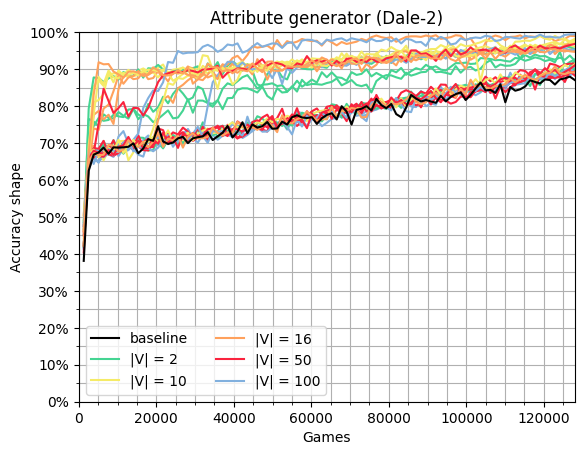
\includegraphics[width=0.485\linewidth]{figures/learning-curve_oh-generator_dale-2_vocab-size.png}
        \label{fig:learning-curve_oh-generator_dale-2_vocab-size}
    }
    \subfigure['Dale-2' dataset with different $n$ highlighted]{
        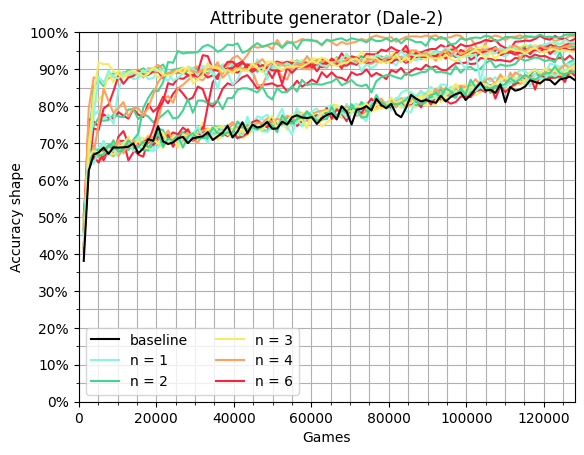
\includegraphics[width=0.485\linewidth]{figures/learning-curve_oh-generator_dale-2_max-len.png}
        \label{fig:learning-curve_oh-generator_dale-2_max-len}
    }
    \subfigure['Dale-5' dataset with different $|V|$ highlighted]{
        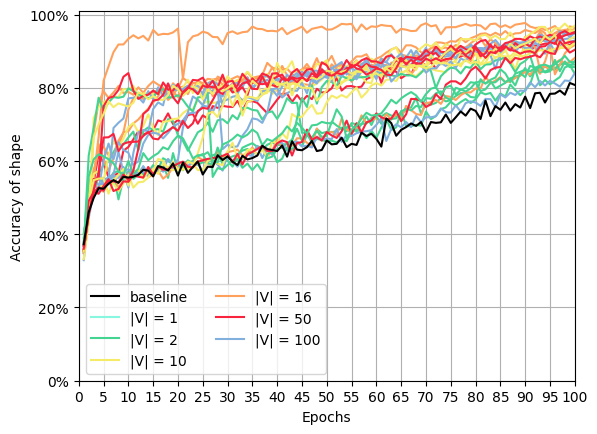
\includegraphics[width=0.485\linewidth]{figures/learning-curve_oh-generator_dale-5_vocab-size.png}
        \label{fig:learning-curve_oh-generator_dale-5_vocab-size}
    }
    \subfigure['Dale-5' dataset with different $n$ highlighted]{
        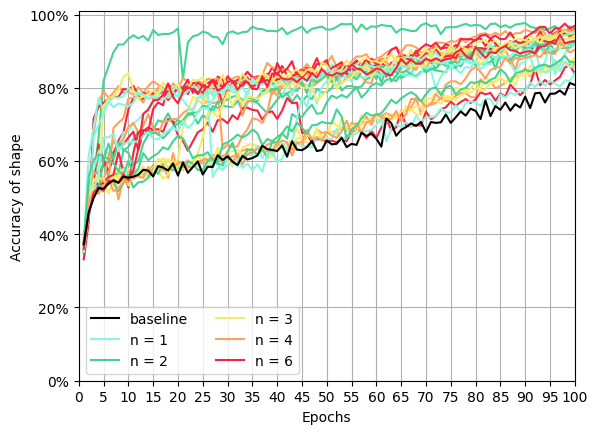
\includegraphics[width=0.485\linewidth]{figures/learning-curve_oh-generator_dale-5_max-len.png}
        \label{fig:learning-curve_oh-generator_dale-5_max-len}
    }
    \caption{Learning curves of all attribute-predictor games on the \emph{Dale} datasets. The graphs show the accuracy of the \emph{shape}, since this highlights the learning effect best. In the left column, the colors correspond to different vocabulary sizes $|V|$ while in the right column, the colors correspond to different message lengths $n$. The baseline is marked in black.}
    \label{fig:learning-curves_oh-generator}
\end{figure}

\begin{table}[ht]
    \centering
    \begin{tabular}{cc|ccc|ccc|ccc}
        \toprule
                                      &         & \multicolumn{3}{c}{\textbf{Dale-2}} & \multicolumn{3}{c}{\textbf{Dale-5}} & \multicolumn{3}{c}{\textbf{CLEVR color}}                                                                                                                                                                                                           \\  \cmidrule(lr){3-5}\cmidrule(lr){6-8}\cmidrule(lr){9-11}
        $n$                           & $|V|$   & \textbf{A\textsubscript{shape}}     & \textbf{A\textsubscript{color}}     & \textbf{A\textsubscript{size}}           & \textbf{A\textsubscript{shape}} & \textbf{A\textsubscript{color}} & \textbf{A\textsubscript{size}} & \textbf{A\textsubscript{shape}} & \textbf{A\textsubscript{color}} & \textbf{A\textsubscript{size}} \\\midrule
        \multicolumn{2}{c|}{baseline} & {88,91} & {92,03}                             & {50,55}                             & {80,78}                                  & {89,38}                         & {49,92}                         & {100}                          & {90,78}                         & {76,72}                                                          \\\midrule
        {1}                           & {2}     & \textcolor{red}{89,69}              & {93,68}                             & \textcolor{red}{52,04}                   & {88,09}                         & \textcolor{red}{90,12}          & \textcolor{red}{49,74}         & {100}                           & \textcolor{red}{87,37}          & \textcolor{red}{76,56}         \\
        {1}                           & {10}    & {96,31}                             & {94,21}                             & \textcolor{red}{52,78}                   & {90,6}                          & \textcolor{red}{90,15}          & \textcolor{red}{49,74}         & {100}                           & \textbf{91,32}                  & \textcolor{red}{76,52}         \\
        {1}                           & {16}    & {94,97}                             & \textcolor{red}{92,8}               & \textcolor{red}{52,78}                   & {91,97}                         & {93,45}                         & \textcolor{red}{49,74}         & {100}                           & \textcolor{red}{91,03}          & \textcolor{red}{76,52}         \\
        {1}                           & {50}    & \textcolor{red}{90,1}               & \textcolor{red}{91,58}              & \textcolor{red}{52,78}                   & {94,66}                         & {93,39}                         & \textcolor{red}{49,74}         & {100}                           & \textcolor{red}{89,41}          & \textcolor{red}{76,52}         \\
        {1}                           & {100}   & {90,41}                             & \textcolor{red}{92,66}              & \textcolor{red}{52,78}                   & \textcolor{red}{83,03}          & \textcolor{red}{90,23}          & \textcolor{red}{49,74}         & {100}                           & \textcolor{red}{86,72}          & \textcolor{red}{76,52}         \\
        {2}                           & {2}     & {92,45}                             & \textcolor{red}{92,45}              & \textcolor{red}{52,04}                   & {88,72}                         & \textbf{94,38}                  & \textcolor{red}{49,74}         & {100}                           & \textcolor{red}{88,89}          & \textcolor{red}{76,56}         \\
        {2}                           & {10}    & {96,09}                             & \textbf{94,44}                      & \textcolor{red}{52,78}                   & {91,54}                         & \textcolor{red}{90,71}          & \textcolor{red}{49,74}         & {100}                           & \textcolor{red}{89,54}          & \textcolor{red}{76,52}         \\
        {2}                           & {16}    & {90,58}                             & \textcolor{red}{92,66}              & \textcolor{red}{52,78}                   & \textbf{97,18}                  & {94,14}                         & \textcolor{red}{49,74}         & {100}                           & \textcolor{red}{86,98}          & \textcolor{red}{76,52}         \\
        {2}                           & {50}    & {89,28}                             & \textcolor{red}{92,45}              & \textcolor{red}{52,78}                   & {92,01}                         & {93,01}                         & \textcolor{red}{49,74}         & {100}                           & \textcolor{red}{86,5}           & \textcolor{red}{76,52}         \\
        {2}                           & {100}   & \textbf{98,91}                      & \textcolor{red}{92,97}              & \textcolor{red}{52,78}                   & {92,66}                         & {92,49}                         & \textcolor{red}{49,74}         & {100}                           & \textcolor{red}{86,68}          & \textcolor{red}{76,52}         \\
        {3}                           & {2}     & {90,97}                             & {93,32}                             & \textcolor{red}{52,04}                   & {87,88}                         & {92,53}                         & \textcolor{red}{49,74}         & {100}                           & \textcolor{red}{90,58}          & \textcolor{red}{76,56}         \\
        {3}                           & {10}    & {97,01}                             & \textbf{{94,79}}                    & \textcolor{red}{52,78}                   & {94,4}                          & {92,8}                          & \textcolor{red}{49,74}         & {100}                           & \textbf{91,17}                  & \textcolor{red}{76,52}         \\
        {3}                           & {16}    & {95,36}                             & {93,1}                              & \textcolor{red}{52,78}                   & {86,72}                         & {91,88}                         & \textcolor{red}{49,74}         & {100}                           & \textcolor{red}{88,06}          & \textcolor{red}{76,52}         \\
        {3}                           & {50}    & {90,93}                             & \textcolor{red}{90,84}              & \textcolor{red}{52,78}                   & {94,92}                         & \textbf{94,18}                  & \textcolor{red}{49,74}         & {100}                           & \textcolor{red}{88,59}          & \textcolor{red}{76,52}         \\
        {3}                           & {100}   & \textcolor{red}{89,37}              & \textcolor{red}{90,76}              & \textcolor{red}{52,78}                   & {94,1}                          & {92,8}                          & \textcolor{red}{49,74}         & {100}                           & \textbf{91,84}                  & \textcolor{red}{76,52}         \\
        {4}                           & {2}     & {94,86}                             & \textcolor{red}{92,11}              & \textcolor{red}{52,04}                   & {88,56}                         & {93,86}                         & \textcolor{red}{49,74}         & {100}                           & \textcolor{red}{87,11}          & \textcolor{red}{76,56}         \\
        {4}                           & {10}    & {90,58}                             & \textcolor{red}{92,75}              & \textcolor{red}{52,78}                   & {95,05}                         & {93,71}                         & \textcolor{red}{49,74}         & {100}                           & \textcolor{red}{89,89}          & \textcolor{red}{76,52}         \\
        {4}                           & {16}    & \textbf{98,57}                      & {94,14}                             & \textcolor{red}{52,78}                   & \textbf{96,14}                  & \textbf{95,23}                  & \textcolor{red}{49,74}         & {100}                           & \textcolor{red}{88,06}          & \textcolor{red}{76,52}         \\
        {4}                           & {50}    & {95,66}                             & {93,32}                             & \textcolor{red}{52,78}                   & {91,01}                         & \textcolor{red}{90,45}          & \textcolor{red}{49,74}         & {100}                           & \textcolor{red}{88,85}          & \textcolor{red}{76,52}         \\
        {4}                           & {100}   & \textcolor{red}{89,41}              & {93,58}                             & \textcolor{red}{52,78}                   & {94,66}                         & {93,19}                         & \textcolor{red}{49,74}         & {100}                           & \textcolor{red}{86,98}          & \textcolor{red}{76,52}         \\
        {6}                           & {2}     & {93,39}                             & {92,94}                             & \textcolor{red}{52,04}                   & \textcolor{red}{82,18}          & {92,16}                         & \textcolor{red}{49,74}         & {100}                           & \textcolor{red}{90,05}          & \textcolor{red}{76,56}         \\
        {6}                           & {10}    & \textbf{98,78}                      & \textbf{94,23}                      & \textcolor{red}{52,78}                   & \textbf{96,79}                  & {92,75}                         & \textcolor{red}{49,74}         & {100}                           & \textcolor{red}{87,67}          & \textcolor{red}{76,52}         \\
        {6}                           & {16}    & {96,96}                             & \textcolor{red}{91,32}              & \textcolor{red}{52,78}                   & {95,57}                         & {93,75}                         & \textcolor{red}{49,74}         & {100}                           & \textcolor{red}{89,37}          & \textcolor{red}{76,52}         \\
        {6}                           & {50}    & \textcolor{red}{88,28}              & \textcolor{red}{91,45}              & \textcolor{red}{52,78}                   & {91,71}                         & \textcolor{red}{86,24}          & \textcolor{red}{49,74}         & {100}                           & \textcolor{red}{88,32}          & \textcolor{red}{76,52}         \\
        {6}                           & {100}   & {94,92}                             & \textcolor{red}{92,45}              & \textcolor{red}{52,78}                   & {95,3}                          & {93,62}                         & \textcolor{red}{49,74}         & {100}                           & \textcolor{red}{89,19}          & \textcolor{red}{76,52}         \\
        \bottomrule
    \end{tabular}
    \caption{Accuracies for each attribute in \% of the attribute predictor after 128.000 games: $n$ are different maximum message lengths and $|V|$ are different vocabulary sizes.}
    \label{tab:results:attribute-predictor-game}
\end{table}

Finally, Figure \ref{fig:learning-curves_oh-generator} shows the learning curves for the \textbf{attribute generator}.
The measure of learning is hereby the accuracy of the \emph{shape}.
The reason for this is that the \emph{size} is not learned at all, while also the \emph{color} diverges only very slightly from baseline.
Communication is therefore impacting mostly the \emph{shape}, and the influence of the vocabulary size and message length is shown in the figures.
On the 'Dale-2' dataset, configuration that learn the \emph{shape} quickly tend to use smaller vocabularies.
However, there are configurations with $|V| \in \{16,10\}$ that need 15.000 to 20.000 games, but outperform the configurations which learned faster.
A similar result is visible for the message length, where shorter messages help the agents to learn faster while longer messages need more games.
Looking at the 'Dale-5' dataset, more configurations are able to learn the \emph{shape}.
Most of the configurations again outperform the baseline already after 5.000 to 10.000 games, but the learning decelerates shortly after.
Interestingly, most of the configurations reach a final accuracy of the \emph{shape} after 128.000 games of 85\% to 97\%.
However, the learning progress is different across the configurations.
Several configurations progress quickly only to around 65\% with a following relatively steep learning over the remaining 120.000 games.
A second group of configurations has an initial learning to around 80\% and then progresses slower.
On configuration even reaches over 95\% after 15.000 games, but then stagnates until the cutoff.
Looking at the vocabulary size and message length, no consistent influence is visible.
However, agents seem to learn slower with $|V| \in \{50,100\}$, while $|V| \in \{2,16\}$ tends to increase the speed.
Opposed, a short message length tends to decrease the speed.

Table \ref{tab:results:attribute-predictor-game} shows the results for the games in which the receiver predicts a multi-hot vector of the attributes.
In the results for the baseline, it can be seen that the receiver can already predict the \emph{shape} and \emph{color}  very well: 88,91\% and 92\% respectively on the 'Dale-2' dataset, 80,78\% and 89,38\% respectively on the 'Dale-5' dataset, and 100\% and 90,78\% respectively on the 'CLEVR color' dataset.
The \emph{size} however corresponds to a random guess on the \emph{Dale} dataset and only achieves 76,72\% on the 'CLEVR color' dataset.
This shows that the receiver can already identify attributes of the target object on their own and discriminate it from the distractors.
However, the size still seems to be an attribute which is difficult to extract from the visual scene.
The increase in performance compared to the generation of referring expression can be explained by two reasons:
First, the complexity of the receiver is greatly reduced.
When only predicting multi-hot vectors, much fewer layers and weights are involved that need to be trained and hence the models can learn the given task.
Secondly, the complexity of the task is reduced as well.
The generation of referring expressions not only includes the learning of the tokens (and their embeddings), but also their order in the referring expression and their salience for the incremental algorithm.
Using multi-hot vectors, both order and salience are irrelevant and only the attributes themselves are needed to be learned.
The goal of these experiments is now to see if the information of the sender improves the predictions of the receiver.

As can be seen in the table, the improvement is dependent on the attributes.
When the agents are trained on the 'Dale-2' dataset, almost all configurations improve the prediction of the shape.
While 11 out of 30 configurations only improve by a maximum of 2\% points, most can predict the \emph{shape} much better, with an accuracy of up to 98,91\%.
A pattern based on the vocabulary size $|V|$ and message length $n$ is however difficult to identify.
A smaller vocabulary size of $|V|=10$ generally fares well, but also a large vocabulary size of $|V|=100$ can help to predict the shape both with short messages ($n=2$) and long messages ($n=6$).
Opposed to the \emph{shape}, the prediction of the \emph{color} can only be improved by a small margin of a maximum of 2,7\% points.
Most of the configurations produce the same or slightly worse results than the baseline.
Again, a vocabulary of $|V|=10$ seems to help the most.
Interestingly, when the agents can only use one token to encode their message ($|V|=2$), an improvement of predictions of the \emph{shape} comes to the expense of the accuracy of the \emph{color} and vice versa.
This indicates that the sender doesn't have enough space to communicate both attributes to the receiver.
Looking at the \emph{size}, a constant improvement of 2\% points across all configurations can be seen.
The final accuracy however still lies slightly above a random guess.

The results are similar when the agents need to describe the 'Dale-5' dataset.
The baseline accuracies of the \emph{shape} and \emph{color} are lower, but can be improved to similar peaks as for the 'Dale-2' dataset.
The highest accuracy for the \emph{shape} lies at 97,18\%, while it lies at 95,23\% for the \emph{color}.
This indicates that the larger number of distractors makes it difficult to focus on the correct object and instead describes distractors when the receiver is on their own.
But when the sender can communicate the correct object, the receiver describes the attributes as well as with fewer distractors.
As before, the predictions of the \emph{size} correspond to a random guess.

Using the 'CLEVR color' dataset, almost no improvements can be seen.
The predictions of the \emph{shape} stay at 100\% accuracy, while the predictions of the \emph{color} get slightly worse for most configurations and if they improve they only improve by maximum 1\% point.
The predictions of the \emph{size} stay the same.
The fact that the sender has a smaller influence on the 'CLEVR color' dataset than on the \emph{Dale} dataset is surprising since the sender would need to communicate only the \emph{color} instead of additionally the \emph{shape} (and \emph{size}).
A reason why this happens might be the larger number of distractors.
This number might hinder the receiver to converge and understand the task, by connecting the multi-hot vector to the colors of the target object.
While for the \emph{Dale} datasets the receiver has a choice between only 2 to 5 objects, they need to decide between up to 10 objects on the 'CLEVR color' dataset.
That might confuse the model where to focus on and subsequently to connect it to the on-hot vector.
Future experiments with a similar dataset including fewer distractors would need to verify this hypothesis.

Concluding, these experiments show that the models are able to extract and communicate information about the \emph{shape} and \emph{color} from the images when few objects are present.
When the agents are forced to generate referring expressions which are more complex in their structure, they produce perfect results less frequently.
However, the communication is successfully very often as it helps the receiver in identifying the correct attributes and referring expression.